% Created by tikzDevice version 0.10.1 on 2018-01-23 20:20:11
% !TEX encoding = UTF-8 Unicode
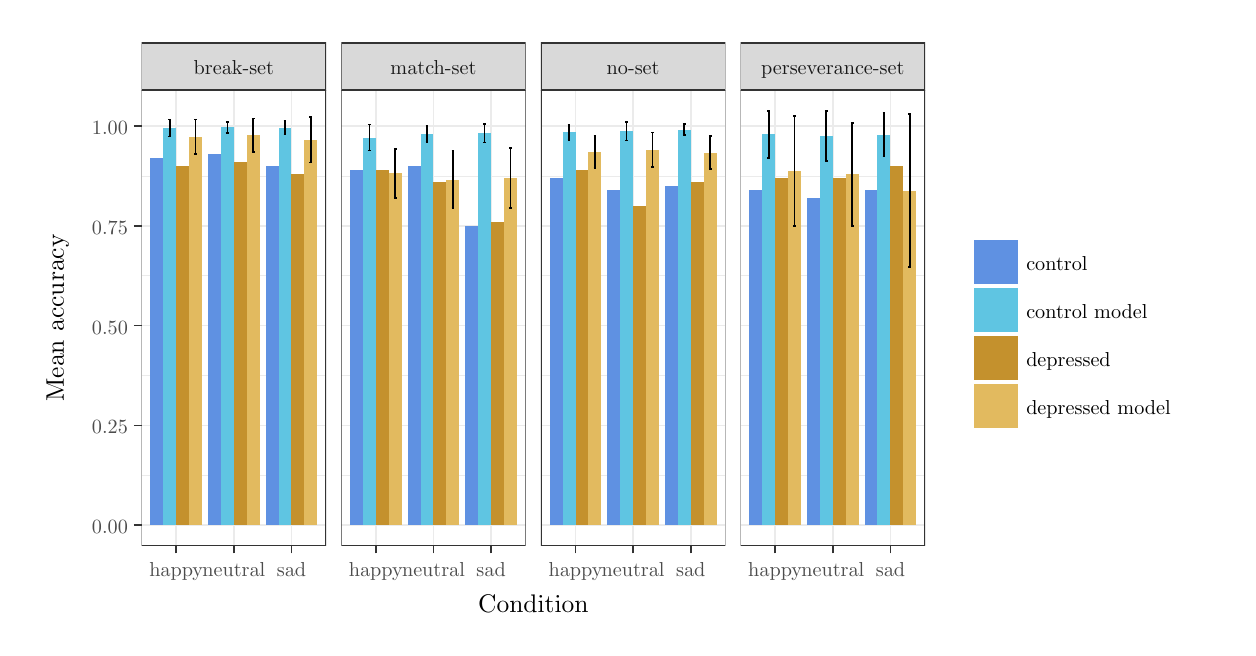
\begin{tikzpicture}[x=1pt,y=1pt]
\definecolor{fillColor}{RGB}{255,255,255}
\path[use as bounding box,fill=fillColor,fill opacity=0.00] (0,0) rectangle (433.62,216.81);
\begin{scope}
\path[clip] (  0.00,  0.00) rectangle (433.62,216.81);
\definecolor{drawColor}{RGB}{255,255,255}
\definecolor{fillColor}{RGB}{255,255,255}

\path[draw=drawColor,line width= 0.6pt,line join=round,line cap=round,fill=fillColor] (  0.00,  0.00) rectangle (433.62,216.81);
\end{scope}
\begin{scope}
\path[clip] ( 41.17, 29.59) rectangle (107.82,194.25);
\definecolor{fillColor}{RGB}{255,255,255}

\path[fill=fillColor] ( 41.17, 29.59) rectangle (107.82,194.25);
\definecolor{drawColor}{gray}{0.92}

\path[draw=drawColor,line width= 0.3pt,line join=round] ( 41.17, 55.09) --
	(107.82, 55.09);

\path[draw=drawColor,line width= 0.3pt,line join=round] ( 41.17, 91.11) --
	(107.82, 91.11);

\path[draw=drawColor,line width= 0.3pt,line join=round] ( 41.17,127.14) --
	(107.82,127.14);

\path[draw=drawColor,line width= 0.3pt,line join=round] ( 41.17,163.17) --
	(107.82,163.17);

\path[draw=drawColor,line width= 0.6pt,line join=round] ( 41.17, 37.07) --
	(107.82, 37.07);

\path[draw=drawColor,line width= 0.6pt,line join=round] ( 41.17, 73.10) --
	(107.82, 73.10);

\path[draw=drawColor,line width= 0.6pt,line join=round] ( 41.17,109.13) --
	(107.82,109.13);

\path[draw=drawColor,line width= 0.6pt,line join=round] ( 41.17,145.15) --
	(107.82,145.15);

\path[draw=drawColor,line width= 0.6pt,line join=round] ( 41.17,181.18) --
	(107.82,181.18);

\path[draw=drawColor,line width= 0.6pt,line join=round] ( 53.67, 29.59) --
	( 53.67,194.25);

\path[draw=drawColor,line width= 0.6pt,line join=round] ( 74.50, 29.59) --
	( 74.50,194.25);

\path[draw=drawColor,line width= 0.6pt,line join=round] ( 95.32, 29.59) --
	( 95.32,194.25);
\definecolor{fillColor}{RGB}{226,186,95}

\path[fill=fillColor] ( 58.36, 37.07) rectangle ( 63.04,177.39);
\definecolor{fillColor}{RGB}{196,145,45}

\path[fill=fillColor] ( 53.67, 37.07) rectangle ( 58.36,166.77);
\definecolor{fillColor}{RGB}{95,197,226}

\path[fill=fillColor] ( 48.98, 37.07) rectangle ( 53.67,180.59);
\definecolor{fillColor}{RGB}{95,145,226}

\path[fill=fillColor] ( 44.30, 37.07) rectangle ( 48.98,169.65);
\definecolor{fillColor}{RGB}{226,186,95}

\path[fill=fillColor] ( 79.18, 37.07) rectangle ( 83.87,177.96);
\definecolor{fillColor}{RGB}{196,145,45}

\path[fill=fillColor] ( 74.50, 37.07) rectangle ( 79.18,168.21);
\definecolor{fillColor}{RGB}{95,197,226}

\path[fill=fillColor] ( 69.81, 37.07) rectangle ( 74.50,180.78);
\definecolor{fillColor}{RGB}{95,145,226}

\path[fill=fillColor] ( 65.12, 37.07) rectangle ( 69.81,171.09);
\definecolor{fillColor}{RGB}{226,186,95}

\path[fill=fillColor] (100.01, 37.07) rectangle (104.69,176.30);
\definecolor{fillColor}{RGB}{196,145,45}

\path[fill=fillColor] ( 95.32, 37.07) rectangle (100.01,163.89);
\definecolor{fillColor}{RGB}{95,197,226}

\path[fill=fillColor] ( 90.64, 37.07) rectangle ( 95.32,180.59);
\definecolor{fillColor}{RGB}{95,145,226}

\path[fill=fillColor] ( 85.95, 37.07) rectangle ( 90.64,166.77);
\definecolor{drawColor}{RGB}{0,0,0}

\path[draw=drawColor,line width= 0.6pt,line join=round] ( 60.18,183.67) --
	( 61.22,183.67);

\path[draw=drawColor,line width= 0.6pt,line join=round] ( 60.70,183.67) --
	( 60.70,171.11);

\path[draw=drawColor,line width= 0.6pt,line join=round] ( 60.18,171.11) --
	( 61.22,171.11);

\path[draw=drawColor,line width= 0.6pt,line join=round] ( 50.81,183.65) --
	( 51.85,183.65);

\path[draw=drawColor,line width= 0.6pt,line join=round] ( 51.33,183.65) --
	( 51.33,177.54);

\path[draw=drawColor,line width= 0.6pt,line join=round] ( 50.81,177.54) --
	( 51.85,177.54);

\path[draw=drawColor,line width= 0.6pt,line join=round] ( 81.00,183.95) --
	( 82.05,183.95);

\path[draw=drawColor,line width= 0.6pt,line join=round] ( 81.52,183.95) --
	( 81.52,171.96);

\path[draw=drawColor,line width= 0.6pt,line join=round] ( 81.00,171.96) --
	( 82.05,171.96);

\path[draw=drawColor,line width= 0.6pt,line join=round] ( 71.63,182.78) --
	( 72.67,182.78);

\path[draw=drawColor,line width= 0.6pt,line join=round] ( 72.15,182.78) --
	( 72.15,178.78);

\path[draw=drawColor,line width= 0.6pt,line join=round] ( 71.63,178.78) --
	( 72.67,178.78);

\path[draw=drawColor,line width= 0.6pt,line join=round] (101.83,184.47) --
	(102.87,184.47);

\path[draw=drawColor,line width= 0.6pt,line join=round] (102.35,184.47) --
	(102.35,168.12);

\path[draw=drawColor,line width= 0.6pt,line join=round] (101.83,168.12) --
	(102.87,168.12);

\path[draw=drawColor,line width= 0.6pt,line join=round] ( 92.46,182.97) --
	( 93.50,182.97);

\path[draw=drawColor,line width= 0.6pt,line join=round] ( 92.98,182.97) --
	( 92.98,178.22);

\path[draw=drawColor,line width= 0.6pt,line join=round] ( 92.46,178.22) --
	( 93.50,178.22);
\definecolor{drawColor}{gray}{0.20}

\path[draw=drawColor,line width= 0.6pt,line join=round,line cap=round] ( 41.17, 29.59) rectangle (107.82,194.25);
\end{scope}
\begin{scope}
\path[clip] (113.32, 29.59) rectangle (179.96,194.25);
\definecolor{fillColor}{RGB}{255,255,255}

\path[fill=fillColor] (113.32, 29.59) rectangle (179.96,194.25);
\definecolor{drawColor}{gray}{0.92}

\path[draw=drawColor,line width= 0.3pt,line join=round] (113.32, 55.09) --
	(179.96, 55.09);

\path[draw=drawColor,line width= 0.3pt,line join=round] (113.32, 91.11) --
	(179.96, 91.11);

\path[draw=drawColor,line width= 0.3pt,line join=round] (113.32,127.14) --
	(179.96,127.14);

\path[draw=drawColor,line width= 0.3pt,line join=round] (113.32,163.17) --
	(179.96,163.17);

\path[draw=drawColor,line width= 0.6pt,line join=round] (113.32, 37.07) --
	(179.96, 37.07);

\path[draw=drawColor,line width= 0.6pt,line join=round] (113.32, 73.10) --
	(179.96, 73.10);

\path[draw=drawColor,line width= 0.6pt,line join=round] (113.32,109.13) --
	(179.96,109.13);

\path[draw=drawColor,line width= 0.6pt,line join=round] (113.32,145.15) --
	(179.96,145.15);

\path[draw=drawColor,line width= 0.6pt,line join=round] (113.32,181.18) --
	(179.96,181.18);

\path[draw=drawColor,line width= 0.6pt,line join=round] (125.81, 29.59) --
	(125.81,194.25);

\path[draw=drawColor,line width= 0.6pt,line join=round] (146.64, 29.59) --
	(146.64,194.25);

\path[draw=drawColor,line width= 0.6pt,line join=round] (167.47, 29.59) --
	(167.47,194.25);
\definecolor{fillColor}{RGB}{226,186,95}

\path[fill=fillColor] (130.50, 37.07) rectangle (135.19,164.18);
\definecolor{fillColor}{RGB}{196,145,45}

\path[fill=fillColor] (125.81, 37.07) rectangle (130.50,165.33);
\definecolor{fillColor}{RGB}{95,197,226}

\path[fill=fillColor] (121.13, 37.07) rectangle (125.81,177.11);
\definecolor{fillColor}{RGB}{95,145,226}

\path[fill=fillColor] (116.44, 37.07) rectangle (121.13,165.33);
\definecolor{fillColor}{RGB}{226,186,95}

\path[fill=fillColor] (151.33, 37.07) rectangle (156.01,161.90);
\definecolor{fillColor}{RGB}{196,145,45}

\path[fill=fillColor] (146.64, 37.07) rectangle (151.33,161.01);
\definecolor{fillColor}{RGB}{95,197,226}

\path[fill=fillColor] (141.95, 37.07) rectangle (146.64,178.46);
\definecolor{fillColor}{RGB}{95,145,226}

\path[fill=fillColor] (137.27, 37.07) rectangle (141.95,166.77);
\definecolor{fillColor}{RGB}{226,186,95}

\path[fill=fillColor] (172.15, 37.07) rectangle (176.84,162.44);
\definecolor{fillColor}{RGB}{196,145,45}

\path[fill=fillColor] (167.47, 37.07) rectangle (172.15,146.60);
\definecolor{fillColor}{RGB}{95,197,226}

\path[fill=fillColor] (162.78, 37.07) rectangle (167.47,178.71);
\definecolor{fillColor}{RGB}{95,145,226}

\path[fill=fillColor] (158.10, 37.07) rectangle (162.78,145.15);
\definecolor{drawColor}{RGB}{0,0,0}

\path[draw=drawColor,line width= 0.6pt,line join=round] (132.32,173.01) --
	(133.36,173.01);

\path[draw=drawColor,line width= 0.6pt,line join=round] (132.84,173.01) --
	(132.84,155.36);

\path[draw=drawColor,line width= 0.6pt,line join=round] (132.32,155.36) --
	(133.36,155.36);

\path[draw=drawColor,line width= 0.6pt,line join=round] (122.95,181.77) --
	(123.99,181.77);

\path[draw=drawColor,line width= 0.6pt,line join=round] (123.47,181.77) --
	(123.47,172.45);

\path[draw=drawColor,line width= 0.6pt,line join=round] (122.95,172.45) --
	(123.99,172.45);

\path[draw=drawColor,line width= 0.6pt,line join=round] (153.15,172.18) --
	(154.19,172.18);

\path[draw=drawColor,line width= 0.6pt,line join=round] (153.67,172.18) --
	(153.67,151.62);

\path[draw=drawColor,line width= 0.6pt,line join=round] (153.15,151.62) --
	(154.19,151.62);

\path[draw=drawColor,line width= 0.6pt,line join=round] (143.78,181.48) --
	(144.82,181.48);

\path[draw=drawColor,line width= 0.6pt,line join=round] (144.30,181.48) --
	(144.30,175.44);

\path[draw=drawColor,line width= 0.6pt,line join=round] (143.78,175.44) --
	(144.82,175.44);

\path[draw=drawColor,line width= 0.6pt,line join=round] (173.98,173.34) --
	(175.02,173.34);

\path[draw=drawColor,line width= 0.6pt,line join=round] (174.50,173.34) --
	(174.50,151.53);

\path[draw=drawColor,line width= 0.6pt,line join=round] (173.98,151.53) --
	(175.02,151.53);

\path[draw=drawColor,line width= 0.6pt,line join=round] (164.60,182.06) --
	(165.64,182.06);

\path[draw=drawColor,line width= 0.6pt,line join=round] (165.12,182.06) --
	(165.12,175.36);

\path[draw=drawColor,line width= 0.6pt,line join=round] (164.60,175.36) --
	(165.64,175.36);
\definecolor{drawColor}{gray}{0.20}

\path[draw=drawColor,line width= 0.6pt,line join=round,line cap=round] (113.32, 29.59) rectangle (179.96,194.25);
\end{scope}
\begin{scope}
\path[clip] (185.46, 29.59) rectangle (252.11,194.25);
\definecolor{fillColor}{RGB}{255,255,255}

\path[fill=fillColor] (185.46, 29.59) rectangle (252.11,194.25);
\definecolor{drawColor}{gray}{0.92}

\path[draw=drawColor,line width= 0.3pt,line join=round] (185.46, 55.09) --
	(252.11, 55.09);

\path[draw=drawColor,line width= 0.3pt,line join=round] (185.46, 91.11) --
	(252.11, 91.11);

\path[draw=drawColor,line width= 0.3pt,line join=round] (185.46,127.14) --
	(252.11,127.14);

\path[draw=drawColor,line width= 0.3pt,line join=round] (185.46,163.17) --
	(252.11,163.17);

\path[draw=drawColor,line width= 0.6pt,line join=round] (185.46, 37.07) --
	(252.11, 37.07);

\path[draw=drawColor,line width= 0.6pt,line join=round] (185.46, 73.10) --
	(252.11, 73.10);

\path[draw=drawColor,line width= 0.6pt,line join=round] (185.46,109.13) --
	(252.11,109.13);

\path[draw=drawColor,line width= 0.6pt,line join=round] (185.46,145.15) --
	(252.11,145.15);

\path[draw=drawColor,line width= 0.6pt,line join=round] (185.46,181.18) --
	(252.11,181.18);

\path[draw=drawColor,line width= 0.6pt,line join=round] (197.96, 29.59) --
	(197.96,194.25);

\path[draw=drawColor,line width= 0.6pt,line join=round] (218.79, 29.59) --
	(218.79,194.25);

\path[draw=drawColor,line width= 0.6pt,line join=round] (239.61, 29.59) --
	(239.61,194.25);
\definecolor{fillColor}{RGB}{226,186,95}

\path[fill=fillColor] (202.64, 37.07) rectangle (207.33,171.92);
\definecolor{fillColor}{RGB}{196,145,45}

\path[fill=fillColor] (197.96, 37.07) rectangle (202.64,165.33);
\definecolor{fillColor}{RGB}{95,197,226}

\path[fill=fillColor] (193.27, 37.07) rectangle (197.96,179.00);
\definecolor{fillColor}{RGB}{95,145,226}

\path[fill=fillColor] (188.59, 37.07) rectangle (193.27,162.45);
\definecolor{fillColor}{RGB}{226,186,95}

\path[fill=fillColor] (223.47, 37.07) rectangle (228.16,172.70);
\definecolor{fillColor}{RGB}{196,145,45}

\path[fill=fillColor] (218.79, 37.07) rectangle (223.47,152.36);
\definecolor{fillColor}{RGB}{95,197,226}

\path[fill=fillColor] (214.10, 37.07) rectangle (218.79,179.33);
\definecolor{fillColor}{RGB}{95,145,226}

\path[fill=fillColor] (209.41, 37.07) rectangle (214.10,158.12);
\definecolor{fillColor}{RGB}{226,186,95}

\path[fill=fillColor] (244.30, 37.07) rectangle (248.98,171.69);
\definecolor{fillColor}{RGB}{196,145,45}

\path[fill=fillColor] (239.61, 37.07) rectangle (244.30,161.01);
\definecolor{fillColor}{RGB}{95,197,226}

\path[fill=fillColor] (234.93, 37.07) rectangle (239.61,179.98);
\definecolor{fillColor}{RGB}{95,145,226}

\path[fill=fillColor] (230.24, 37.07) rectangle (234.93,159.57);
\definecolor{drawColor}{RGB}{0,0,0}

\path[draw=drawColor,line width= 0.6pt,line join=round] (204.47,177.81) --
	(205.51,177.81);

\path[draw=drawColor,line width= 0.6pt,line join=round] (204.99,177.81) --
	(204.99,166.03);

\path[draw=drawColor,line width= 0.6pt,line join=round] (204.47,166.03) --
	(205.51,166.03);

\path[draw=drawColor,line width= 0.6pt,line join=round] (195.10,181.79) --
	(196.14,181.79);

\path[draw=drawColor,line width= 0.6pt,line join=round] (195.62,181.79) --
	(195.62,176.20);

\path[draw=drawColor,line width= 0.6pt,line join=round] (195.10,176.20) --
	(196.14,176.20);

\path[draw=drawColor,line width= 0.6pt,line join=round] (225.29,178.95) --
	(226.34,178.95);

\path[draw=drawColor,line width= 0.6pt,line join=round] (225.81,178.95) --
	(225.81,166.44);

\path[draw=drawColor,line width= 0.6pt,line join=round] (225.29,166.44) --
	(226.34,166.44);

\path[draw=drawColor,line width= 0.6pt,line join=round] (215.92,182.61) --
	(216.96,182.61);

\path[draw=drawColor,line width= 0.6pt,line join=round] (216.44,182.61) --
	(216.44,176.06);

\path[draw=drawColor,line width= 0.6pt,line join=round] (215.92,176.06) --
	(216.96,176.06);

\path[draw=drawColor,line width= 0.6pt,line join=round] (246.12,177.66) --
	(247.16,177.66);

\path[draw=drawColor,line width= 0.6pt,line join=round] (246.64,177.66) --
	(246.64,165.72);

\path[draw=drawColor,line width= 0.6pt,line join=round] (246.12,165.72) --
	(247.16,165.72);

\path[draw=drawColor,line width= 0.6pt,line join=round] (236.75,182.04) --
	(237.79,182.04);

\path[draw=drawColor,line width= 0.6pt,line join=round] (237.27,182.04) --
	(237.27,177.92);

\path[draw=drawColor,line width= 0.6pt,line join=round] (236.75,177.92) --
	(237.79,177.92);
\definecolor{drawColor}{gray}{0.20}

\path[draw=drawColor,line width= 0.6pt,line join=round,line cap=round] (185.46, 29.59) rectangle (252.11,194.25);
\end{scope}
\begin{scope}
\path[clip] (257.61, 29.59) rectangle (324.25,194.25);
\definecolor{fillColor}{RGB}{255,255,255}

\path[fill=fillColor] (257.61, 29.59) rectangle (324.25,194.25);
\definecolor{drawColor}{gray}{0.92}

\path[draw=drawColor,line width= 0.3pt,line join=round] (257.61, 55.09) --
	(324.25, 55.09);

\path[draw=drawColor,line width= 0.3pt,line join=round] (257.61, 91.11) --
	(324.25, 91.11);

\path[draw=drawColor,line width= 0.3pt,line join=round] (257.61,127.14) --
	(324.25,127.14);

\path[draw=drawColor,line width= 0.3pt,line join=round] (257.61,163.17) --
	(324.25,163.17);

\path[draw=drawColor,line width= 0.6pt,line join=round] (257.61, 37.07) --
	(324.25, 37.07);

\path[draw=drawColor,line width= 0.6pt,line join=round] (257.61, 73.10) --
	(324.25, 73.10);

\path[draw=drawColor,line width= 0.6pt,line join=round] (257.61,109.13) --
	(324.25,109.13);

\path[draw=drawColor,line width= 0.6pt,line join=round] (257.61,145.15) --
	(324.25,145.15);

\path[draw=drawColor,line width= 0.6pt,line join=round] (257.61,181.18) --
	(324.25,181.18);

\path[draw=drawColor,line width= 0.6pt,line join=round] (270.10, 29.59) --
	(270.10,194.25);

\path[draw=drawColor,line width= 0.6pt,line join=round] (290.93, 29.59) --
	(290.93,194.25);

\path[draw=drawColor,line width= 0.6pt,line join=round] (311.76, 29.59) --
	(311.76,194.25);
\definecolor{fillColor}{RGB}{226,186,95}

\path[fill=fillColor] (274.79, 37.07) rectangle (279.48,165.03);
\definecolor{fillColor}{RGB}{196,145,45}

\path[fill=fillColor] (270.10, 37.07) rectangle (274.79,162.45);
\definecolor{fillColor}{RGB}{95,197,226}

\path[fill=fillColor] (265.42, 37.07) rectangle (270.10,178.21);
\definecolor{fillColor}{RGB}{95,145,226}

\path[fill=fillColor] (260.73, 37.07) rectangle (265.42,158.12);
\definecolor{fillColor}{RGB}{226,186,95}

\path[fill=fillColor] (295.62, 37.07) rectangle (300.30,163.79);
\definecolor{fillColor}{RGB}{196,145,45}

\path[fill=fillColor] (290.93, 37.07) rectangle (295.62,162.45);
\definecolor{fillColor}{RGB}{95,197,226}

\path[fill=fillColor] (286.24, 37.07) rectangle (290.93,177.68);
\definecolor{fillColor}{RGB}{95,145,226}

\path[fill=fillColor] (281.56, 37.07) rectangle (286.24,155.24);
\definecolor{fillColor}{RGB}{226,186,95}

\path[fill=fillColor] (316.44, 37.07) rectangle (321.13,157.89);
\definecolor{fillColor}{RGB}{196,145,45}

\path[fill=fillColor] (311.76, 37.07) rectangle (316.44,166.77);
\definecolor{fillColor}{RGB}{95,197,226}

\path[fill=fillColor] (307.07, 37.07) rectangle (311.76,178.13);
\definecolor{fillColor}{RGB}{95,145,226}

\path[fill=fillColor] (302.39, 37.07) rectangle (307.07,158.12);
\definecolor{drawColor}{RGB}{0,0,0}

\path[draw=drawColor,line width= 0.6pt,line join=round] (276.61,184.83) --
	(277.65,184.83);

\path[draw=drawColor,line width= 0.6pt,line join=round] (277.13,184.83) --
	(277.13,145.22);

\path[draw=drawColor,line width= 0.6pt,line join=round] (276.61,145.22) --
	(277.65,145.22);

\path[draw=drawColor,line width= 0.6pt,line join=round] (267.24,186.76) --
	(268.28,186.76);

\path[draw=drawColor,line width= 0.6pt,line join=round] (267.76,186.76) --
	(267.76,169.65);

\path[draw=drawColor,line width= 0.6pt,line join=round] (267.24,169.65) --
	(268.28,169.65);

\path[draw=drawColor,line width= 0.6pt,line join=round] (297.44,182.39) --
	(298.48,182.39);

\path[draw=drawColor,line width= 0.6pt,line join=round] (297.96,182.39) --
	(297.96,145.18);

\path[draw=drawColor,line width= 0.6pt,line join=round] (297.44,145.18) --
	(298.48,145.18);

\path[draw=drawColor,line width= 0.6pt,line join=round] (288.07,186.63) --
	(289.11,186.63);

\path[draw=drawColor,line width= 0.6pt,line join=round] (288.59,186.63) --
	(288.59,168.73);

\path[draw=drawColor,line width= 0.6pt,line join=round] (288.07,168.73) --
	(289.11,168.73);

\path[draw=drawColor,line width= 0.6pt,line join=round] (318.27,185.50) --
	(319.31,185.50);

\path[draw=drawColor,line width= 0.6pt,line join=round] (318.79,185.50) --
	(318.79,130.27);

\path[draw=drawColor,line width= 0.6pt,line join=round] (318.27,130.27) --
	(319.31,130.27);

\path[draw=drawColor,line width= 0.6pt,line join=round] (308.89,186.02) --
	(309.93,186.02);

\path[draw=drawColor,line width= 0.6pt,line join=round] (309.41,186.02) --
	(309.41,170.24);

\path[draw=drawColor,line width= 0.6pt,line join=round] (308.89,170.24) --
	(309.93,170.24);
\definecolor{drawColor}{gray}{0.20}

\path[draw=drawColor,line width= 0.6pt,line join=round,line cap=round] (257.61, 29.59) rectangle (324.25,194.25);
\end{scope}
\begin{scope}
\path[clip] ( 41.17,194.25) rectangle (107.82,211.31);
\definecolor{drawColor}{gray}{0.20}
\definecolor{fillColor}{gray}{0.85}

\path[draw=drawColor,line width= 0.6pt,line join=round,line cap=round,fill=fillColor] ( 41.17,194.25) rectangle (107.82,211.31);
\definecolor{drawColor}{gray}{0.10}

\node[text=drawColor,anchor=base,inner sep=0pt, outer sep=0pt, scale=  0.73] at ( 74.50,199.75) {break-set};
\end{scope}
\begin{scope}
\path[clip] (113.32,194.25) rectangle (179.96,211.31);
\definecolor{drawColor}{gray}{0.20}
\definecolor{fillColor}{gray}{0.85}

\path[draw=drawColor,line width= 0.6pt,line join=round,line cap=round,fill=fillColor] (113.32,194.25) rectangle (179.96,211.31);
\definecolor{drawColor}{gray}{0.10}

\node[text=drawColor,anchor=base,inner sep=0pt, outer sep=0pt, scale=  0.73] at (146.64,199.75) {match-set};
\end{scope}
\begin{scope}
\path[clip] (185.46,194.25) rectangle (252.11,211.31);
\definecolor{drawColor}{gray}{0.20}
\definecolor{fillColor}{gray}{0.85}

\path[draw=drawColor,line width= 0.6pt,line join=round,line cap=round,fill=fillColor] (185.46,194.25) rectangle (252.11,211.31);
\definecolor{drawColor}{gray}{0.10}

\node[text=drawColor,anchor=base,inner sep=0pt, outer sep=0pt, scale=  0.73] at (218.79,199.75) {no-set};
\end{scope}
\begin{scope}
\path[clip] (257.61,194.25) rectangle (324.25,211.31);
\definecolor{drawColor}{gray}{0.20}
\definecolor{fillColor}{gray}{0.85}

\path[draw=drawColor,line width= 0.6pt,line join=round,line cap=round,fill=fillColor] (257.61,194.25) rectangle (324.25,211.31);
\definecolor{drawColor}{gray}{0.10}

\node[text=drawColor,anchor=base,inner sep=0pt, outer sep=0pt, scale=  0.73] at (290.93,199.75) {perseverance-set};
\end{scope}
\begin{scope}
\path[clip] (  0.00,  0.00) rectangle (433.62,216.81);
\definecolor{drawColor}{gray}{0.20}

\path[draw=drawColor,line width= 0.6pt,line join=round] ( 53.67, 26.84) --
	( 53.67, 29.59);

\path[draw=drawColor,line width= 0.6pt,line join=round] ( 74.50, 26.84) --
	( 74.50, 29.59);

\path[draw=drawColor,line width= 0.6pt,line join=round] ( 95.32, 26.84) --
	( 95.32, 29.59);
\end{scope}
\begin{scope}
\path[clip] (  0.00,  0.00) rectangle (433.62,216.81);
\definecolor{drawColor}{gray}{0.30}

\node[text=drawColor,anchor=base,inner sep=0pt, outer sep=0pt, scale=  0.73] at ( 53.67, 18.58) {happy};

\node[text=drawColor,anchor=base,inner sep=0pt, outer sep=0pt, scale=  0.73] at ( 74.50, 18.58) {neutral};

\node[text=drawColor,anchor=base,inner sep=0pt, outer sep=0pt, scale=  0.73] at ( 95.32, 18.58) {sad};
\end{scope}
\begin{scope}
\path[clip] (  0.00,  0.00) rectangle (433.62,216.81);
\definecolor{drawColor}{gray}{0.20}

\path[draw=drawColor,line width= 0.6pt,line join=round] (125.81, 26.84) --
	(125.81, 29.59);

\path[draw=drawColor,line width= 0.6pt,line join=round] (146.64, 26.84) --
	(146.64, 29.59);

\path[draw=drawColor,line width= 0.6pt,line join=round] (167.47, 26.84) --
	(167.47, 29.59);
\end{scope}
\begin{scope}
\path[clip] (  0.00,  0.00) rectangle (433.62,216.81);
\definecolor{drawColor}{gray}{0.30}

\node[text=drawColor,anchor=base,inner sep=0pt, outer sep=0pt, scale=  0.73] at (125.81, 18.58) {happy};

\node[text=drawColor,anchor=base,inner sep=0pt, outer sep=0pt, scale=  0.73] at (146.64, 18.58) {neutral};

\node[text=drawColor,anchor=base,inner sep=0pt, outer sep=0pt, scale=  0.73] at (167.47, 18.58) {sad};
\end{scope}
\begin{scope}
\path[clip] (  0.00,  0.00) rectangle (433.62,216.81);
\definecolor{drawColor}{gray}{0.20}

\path[draw=drawColor,line width= 0.6pt,line join=round] (197.96, 26.84) --
	(197.96, 29.59);

\path[draw=drawColor,line width= 0.6pt,line join=round] (218.79, 26.84) --
	(218.79, 29.59);

\path[draw=drawColor,line width= 0.6pt,line join=round] (239.61, 26.84) --
	(239.61, 29.59);
\end{scope}
\begin{scope}
\path[clip] (  0.00,  0.00) rectangle (433.62,216.81);
\definecolor{drawColor}{gray}{0.30}

\node[text=drawColor,anchor=base,inner sep=0pt, outer sep=0pt, scale=  0.73] at (197.96, 18.58) {happy};

\node[text=drawColor,anchor=base,inner sep=0pt, outer sep=0pt, scale=  0.73] at (218.79, 18.58) {neutral};

\node[text=drawColor,anchor=base,inner sep=0pt, outer sep=0pt, scale=  0.73] at (239.61, 18.58) {sad};
\end{scope}
\begin{scope}
\path[clip] (  0.00,  0.00) rectangle (433.62,216.81);
\definecolor{drawColor}{gray}{0.20}

\path[draw=drawColor,line width= 0.6pt,line join=round] (270.10, 26.84) --
	(270.10, 29.59);

\path[draw=drawColor,line width= 0.6pt,line join=round] (290.93, 26.84) --
	(290.93, 29.59);

\path[draw=drawColor,line width= 0.6pt,line join=round] (311.76, 26.84) --
	(311.76, 29.59);
\end{scope}
\begin{scope}
\path[clip] (  0.00,  0.00) rectangle (433.62,216.81);
\definecolor{drawColor}{gray}{0.30}

\node[text=drawColor,anchor=base,inner sep=0pt, outer sep=0pt, scale=  0.73] at (270.10, 18.58) {happy};

\node[text=drawColor,anchor=base,inner sep=0pt, outer sep=0pt, scale=  0.73] at (290.93, 18.58) {neutral};

\node[text=drawColor,anchor=base,inner sep=0pt, outer sep=0pt, scale=  0.73] at (311.76, 18.58) {sad};
\end{scope}
\begin{scope}
\path[clip] (  0.00,  0.00) rectangle (433.62,216.81);
\definecolor{drawColor}{gray}{0.30}

\node[text=drawColor,anchor=base east,inner sep=0pt, outer sep=0pt, scale=  0.73] at ( 36.22, 34.04) {0.00};

\node[text=drawColor,anchor=base east,inner sep=0pt, outer sep=0pt, scale=  0.73] at ( 36.22, 70.07) {0.25};

\node[text=drawColor,anchor=base east,inner sep=0pt, outer sep=0pt, scale=  0.73] at ( 36.22,106.10) {0.50};

\node[text=drawColor,anchor=base east,inner sep=0pt, outer sep=0pt, scale=  0.73] at ( 36.22,142.12) {0.75};

\node[text=drawColor,anchor=base east,inner sep=0pt, outer sep=0pt, scale=  0.73] at ( 36.22,178.15) {1.00};
\end{scope}
\begin{scope}
\path[clip] (  0.00,  0.00) rectangle (433.62,216.81);
\definecolor{drawColor}{gray}{0.20}

\path[draw=drawColor,line width= 0.6pt,line join=round] ( 38.42, 37.07) --
	( 41.17, 37.07);

\path[draw=drawColor,line width= 0.6pt,line join=round] ( 38.42, 73.10) --
	( 41.17, 73.10);

\path[draw=drawColor,line width= 0.6pt,line join=round] ( 38.42,109.13) --
	( 41.17,109.13);

\path[draw=drawColor,line width= 0.6pt,line join=round] ( 38.42,145.15) --
	( 41.17,145.15);

\path[draw=drawColor,line width= 0.6pt,line join=round] ( 38.42,181.18) --
	( 41.17,181.18);
\end{scope}
\begin{scope}
\path[clip] (  0.00,  0.00) rectangle (433.62,216.81);
\definecolor{drawColor}{RGB}{0,0,0}

\node[text=drawColor,anchor=base,inner sep=0pt, outer sep=0pt, scale=  0.92] at (182.71,  5.50) {Condition};
\end{scope}
\begin{scope}
\path[clip] (  0.00,  0.00) rectangle (433.62,216.81);
\definecolor{drawColor}{RGB}{0,0,0}

\node[text=drawColor,rotate= 90.00,anchor=base,inner sep=0pt, outer sep=0pt, scale=  0.92] at ( 13.08,111.92) {Mean accuracy};
\end{scope}
\begin{scope}
\path[clip] (  0.00,  0.00) rectangle (433.62,216.81);
\definecolor{fillColor}{RGB}{255,255,255}

\path[fill=fillColor] (335.63, 65.58) rectangle (428.12,158.25);
\end{scope}
\begin{scope}
\path[clip] (  0.00,  0.00) rectangle (433.62,216.81);
\definecolor{fillColor}{RGB}{255,255,255}

\path[fill=fillColor] (341.32,123.31) rectangle (358.67,140.65);
\end{scope}
\begin{scope}
\path[clip] (  0.00,  0.00) rectangle (433.62,216.81);
\definecolor{fillColor}{RGB}{95,145,226}

\path[fill=fillColor] (342.04,124.02) rectangle (357.96,139.94);
\end{scope}
\begin{scope}
\path[clip] (  0.00,  0.00) rectangle (433.62,216.81);
\definecolor{fillColor}{RGB}{255,255,255}

\path[fill=fillColor] (341.32,105.96) rectangle (358.67,123.31);
\end{scope}
\begin{scope}
\path[clip] (  0.00,  0.00) rectangle (433.62,216.81);
\definecolor{fillColor}{RGB}{95,197,226}

\path[fill=fillColor] (342.04,106.67) rectangle (357.96,122.60);
\end{scope}
\begin{scope}
\path[clip] (  0.00,  0.00) rectangle (433.62,216.81);
\definecolor{fillColor}{RGB}{255,255,255}

\path[fill=fillColor] (341.32, 88.62) rectangle (358.67,105.96);
\end{scope}
\begin{scope}
\path[clip] (  0.00,  0.00) rectangle (433.62,216.81);
\definecolor{fillColor}{RGB}{196,145,45}

\path[fill=fillColor] (342.04, 89.33) rectangle (357.96,105.25);
\end{scope}
\begin{scope}
\path[clip] (  0.00,  0.00) rectangle (433.62,216.81);
\definecolor{fillColor}{RGB}{255,255,255}

\path[fill=fillColor] (341.32, 71.27) rectangle (358.67, 88.62);
\end{scope}
\begin{scope}
\path[clip] (  0.00,  0.00) rectangle (433.62,216.81);
\definecolor{fillColor}{RGB}{226,186,95}

\path[fill=fillColor] (342.04, 71.98) rectangle (357.96, 87.91);
\end{scope}
\begin{scope}
\path[clip] (  0.00,  0.00) rectangle (433.62,216.81);
\definecolor{drawColor}{RGB}{0,0,0}

\node[text=drawColor,anchor=base west,inner sep=0pt, outer sep=0pt, scale=  0.73] at (360.84,128.95) {control};
\end{scope}
\begin{scope}
\path[clip] (  0.00,  0.00) rectangle (433.62,216.81);
\definecolor{drawColor}{RGB}{0,0,0}

\node[text=drawColor,anchor=base west,inner sep=0pt, outer sep=0pt, scale=  0.73] at (360.84,111.60) {control model};
\end{scope}
\begin{scope}
\path[clip] (  0.00,  0.00) rectangle (433.62,216.81);
\definecolor{drawColor}{RGB}{0,0,0}

\node[text=drawColor,anchor=base west,inner sep=0pt, outer sep=0pt, scale=  0.73] at (360.84, 94.26) {depressed};
\end{scope}
\begin{scope}
\path[clip] (  0.00,  0.00) rectangle (433.62,216.81);
\definecolor{drawColor}{RGB}{0,0,0}

\node[text=drawColor,anchor=base west,inner sep=0pt, outer sep=0pt, scale=  0.73] at (360.84, 76.91) {depressed model};
\end{scope}
\end{tikzpicture}
